
\documentclass[a4paper,kul]{kulakarticle} %options: kul or kulak (default)

\usepackage[utf8]{inputenc}
\usepackage[dutch]{babel}
\usepackage{graphicx}
\usepackage{hyperref}
\usepackage{subcaption}

\date{31/05/2019}
\address{
  Faculteit Industriële Ingenieurswetenschappen \\
  Projectlab bachelor elektronica-ICT \\
  J. Lannoo, L. Espeel}
\title{Verslag E-ink room reservation display}
\author{Baptiste Pattyn\and Michel Dequick \and Stijn Declerck \and Ine Vanderhaeghe}


\begin{document}

\maketitle

\begin{center}
	\centering
	\vspace*{\fill}
	\huge
	\textbf{E-ink room reservation display}
	\vspace*{\fill}
\end{center}

\newpage

\section{Inhoud}

\tableofcontents

\newpage

\section{Probleemstelling}

We willen een display maken voor klaslokalen die dynamisch kan veranderen per uur. 

Op het scherm moeten verschillende zaken komen: het nummer van het klaslokaal, de datum, op welke uren het lokaal bezet is op die dag, welk vak op dit moment gegeven wordt en de docent die dit vak geeft.
\newline

Er zijn verschillende dingen waar we rekening mee moeten houden om dit te realiseren:

We moeten een E-ink display implementeren. Hierbij moeten we bekijken als hier burn-in of ghosting kan optreden. Ook moeten we rekening houden met de grootte van de memory in de display. 

Er moet een databank opgezet worden waar alle data van de lokalen in opgeslagen is. Deze databank moet bereikbaar zijn via wifi.

Er moet een connectie gemaakt worden via een wifi module van de databank naar de display.
\newline

We gebruiken hiervoor een E-ink display omdat dit het meest energiezuinig is. Dit komt omdat de display enkel voeding nodig heeft om het scherm te veranderen. We moeten het scherm maar om het uur aanpassen, dus alle tijd daartussen heeft een E-ink display geen voeding nodig.
Een ander voordeel van een E-ink display is dat het geen licht uitzendt, maar het reflecteert licht zoals een blad papier. Hierdoor is het gemakkelijker leesbaar, ook als er in de omgeving veel licht is. 
\newline

De eenvoudigste E-ink display is de "two pigment ink system". Dit bestaat uit kleine gebieden die dipolen zijn (deze worden gebruikt als de pixels van de afbeelding). De positieve kant van de gebieden bestaat uit wit pigment, de negatieve kant is zwart pigment. Deze gebieden bevinden zich in een bubbel van olie zodat ze gemakkelijk kunnen omdraaien, en zitten tussen transparante elektrode lagen. Wanneer nu op die elektrode lagen een spanning wordt gezet, kan bepaald worden welke delen van het scherm zwart zijn, en welke wit. Op die manier kan een zwart-wit afbeelding op de display geprogrammeerd worden. (zie afbeelding \ref{fig:2psystem} ).

\begin{figure}[h!]
	\centering
	\begin{subfigure}{.5\textwidth}
		\centering
		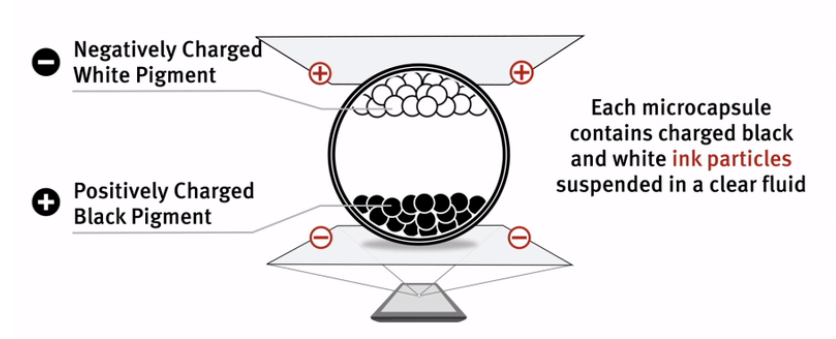
\includegraphics[width=0.95\textwidth]{Two_pigment_ink_system1}
		\label{fig:sub2psystem}
	\end{subfigure}%
	\begin{subfigure}{.5\textwidth}
		\centering
		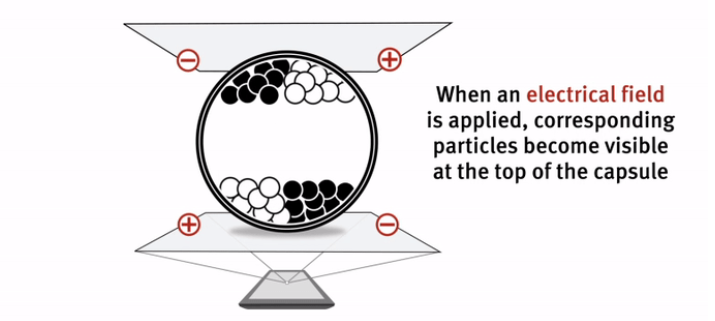
\includegraphics[width=0.95\textwidth]{Two_pigment_ink_system2}
		\label{fig:sub2psystem2}
	\end{subfigure}
	\caption{two pigment ink system}
	\label{fig:2psystem}
\end{figure}

Er bestaat ook een "Three pigment ink system". Dit werkt op ongeveer dezelfde manier als two pigment ink system (zie afbeelding \ref{fig:3psystem} ). Hier is het witte pigment negatief geladen en het rode pigment is positief geladen. Om het zwarte pigment aan de oppervlakte te brengen, moet er een gesplitste lading aangebracht worden.

\begin{figure}[h!]
	\centering
	\begin{subfigure}{.5\textwidth}
		\centering
		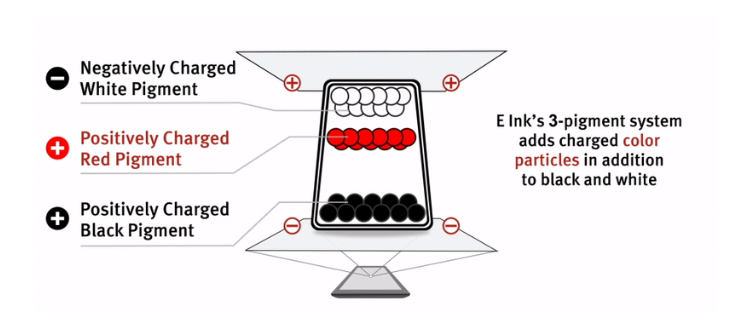
\includegraphics[width=0.95\textwidth]{three_pigment_ink_system1}
		\label{fig:sub3psystem}
	\end{subfigure}%
	\begin{subfigure}{.5\textwidth}
		\centering
		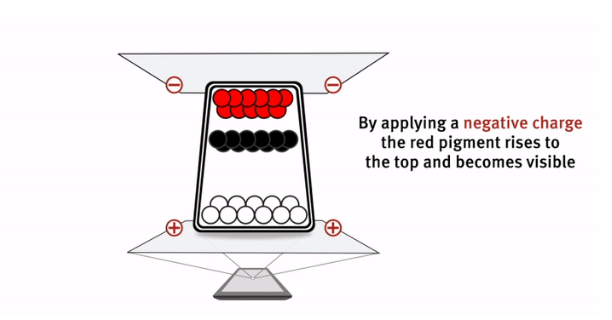
\includegraphics[width=0.95\textwidth]{three_pigment_ink_system2}
		\label{fig:sub3psystem2}
	\end{subfigure}
	\caption{three pigment ink system}
	\label{fig:3psystem}
\end{figure}

De E-ink display die wij gaan gebruiken, gebruikt het three pigment ink system. Op deze manier kunnen we op een overzichtelijke manier op een tijdslijn aanduiden op welke uren het lokaal bezet is.
\newline

Daarnaast bestaat er ook een "Advanced color ePaper". Hierbij kunnen nog meer kleuren op het scherm afgebeeld worden. (zie afbeelding \ref{fig:ACeP} ). Dit gebruiken wij niet in dit project. Dit systeem gebruikt 4 kleuren: cyaan, magenta, geel en wit.  \newline

\begin{figure}[h!]
	\centering
	\begin{subfigure}{.5\textwidth}
		\centering
		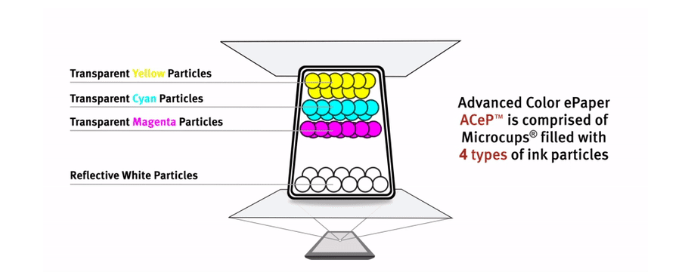
\includegraphics[width=0.95\textwidth]{ACeP1}
		\label{fig:subACeP}
	\end{subfigure}%
	\begin{subfigure}{.5\textwidth}
		\centering
		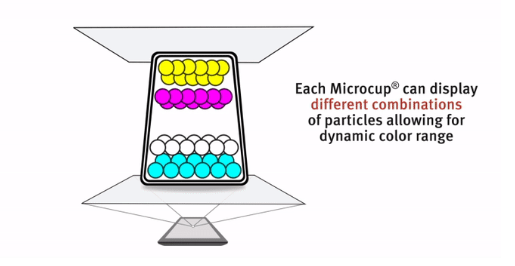
\includegraphics[width=0.95\textwidth]{ACeP2}
		\label{fig:subACeP2}
	\end{subfigure}
	\caption{Advanced color ePaper}
	\label{fig:ACeP}
\end{figure}

bron figuren: \cite{E-ink}.

bron werking ACeP: \cite{ACeP}.
\newline
\newline
Dit is het materiaal dat we gebruikt hebben:
\newline
Mbed FRDM-K64F

met application shield en click shield
\newline
ESP-WROOM-02 click met ESP8266EX wifi bord

Datasheet ESP-WROOM-02: \cite{ESP-WROOM-02}

Datasheet ESP8266EX: \cite{ESP8266EX}
\newline
Eink click, small and big display

\newpage

\section{Aanpak}

Eerst hebben we alle deelopdrachten op een rijtje gezet en een planning gemaakt. Daarbij hebben we ook een taakverdeling gemaakt. 
\newline
\newline
Dit zijn de grootste taken:
\newline
\newline
Een library maken voor de display – Michel
\newline
Eerst moesten we bekijken hoe we een afbeelding op de display konden krijgen. Op het internet vonden we een voorbeeld van een E-ink display die gemaakt was met een Arduino. Wij maken gebruik van een mbed, dus we hebben de code moeten aanpassen. 
Als eerste hebben we geprobeerd om een afbeelding op de display te zetten en om een afbeelding die er op staat te kunnen wissen.
Daarna hebben we een ontwerp gemaakt van wat we allemaal op het scherm wilden zetten en waar. We hebben dan ook geprobeerd om dit op de display te krijgen.
\newline
\newline
Een database opstellen met een wifi access point – Baptiste
\newline
We hebben een database opgesteld op een Raspberry Pi. Daar hebben we ook een wifi access point op geïmplementeerd zodat de display met de databank kan communiceren.
Eens de databank opgevuld was konden we testen als we de data konden in een tabel zetten per lokaal.
\newline
\newline
Wifi connectiviteit maken – Stijn
\newline
Het is belangrijk om via wifi te kunnen communiceren tussen de E-ink display en de databank. Hiervoor moesten we onderzoeken hoe een HTTP GET request werkt en het hoe we het zelf konden implementeren in onze toepassing.
\newline
\newline
Er waren ook enkele kleinere taken.
\newline
\newline
De databank invullen – Ine
\newline
De databank moest opgevuld worden met fictieve data over de lokaalbezetting zodat we een proof of concept konden maken om voor te stellen op de presentatie van ons project.
\newline
\newline
Het verslag en de powerpointpresentatie opstarten – Ine 
\newline
Om het verslag te maken heeft iedereen het deel ingevuld waar hij zelf meest aan gewerkt heeft aangevuld. 

\newpage

\section{Implementatie}
\subsection{Database en Wifi Access Point}
Voor het opslaan van de gegevens is er een database opgezet op een Raspberry Pi model B+ door gebruik te maken van phpMyAdmin. Hier draait een SQL server op waarin alle gegevens voor de komende events van verschillende lokalen kunnen opgeslagen worden. Verder zijn alle gegevens van de courses er ook opgeslagen en de algemene info van de rooms. Om ervoor te zorgen dat onze MBED toegang kan krijgen tot deze database hebben we een Wifi Access Point (WAP) op de Raspberry Pi gezet, waarmee de MBED zich kan verbinden via een ESP8266 Wifi chip. Het opvragen van de gegevens door de mbed gebeurt via een GET request op de HTTP poort van de Raspberry Pi (poort 80).
 
\subsubsection{Database}
Deze database genaamd roomdb bestaat uit 3 verschillende tables: courses, events en rooms. De structuur van de database en de relaties tussen de verschillende tables staat afgebeeld in figuur \ref{fig:dbstruct}. Op de Raspberry Pi staan verschillende PHP files die ervoor zorgen dat de webserver kan verbinden met de database. Een belangrijke file hierbij is dbConnect.php \ref{fig:dbconnect}, in deze file staan de gegevens die nodig zijn om te kunnen verbinden met de database. In deze  file declareren we verschillende variabelen: \verb|$host|, \verb|$user|, \verb|$password|en \verb|$databse|. Deze worden dan gebruikt in een \verb|mysqli_connect()| commando om een verbinding op te zetten met de databse. Hierna wordt er nog een controle gedaan om te kijken of de verbinding tot stand is gekomen, indien dit niet het geval is dan verkrijgen we een error. Deze code is enkel bedoeld voor tijdens het opzetten van de webserver en de database en dient verwijderd te worden indien de code definitief in gebruik wordt genomen. Als \verb|$host| kiezen we het local host adres 127.0.0.1 omdat de database zich op de Raspberry Pi zelf bevindt. De \verb|$user| en het \verb|$password| zijn specifiek voor elke database en hangen af van welke user je ingesteld hebt op je SQL server. 
\begin{figure}[h]
	\begin{verbatim}
	<?php
	$host = "127.0.0.1";
	$user = "root";
	$password = "password" ;
	$database = "roomdb";
	$conn = mysqli_connect($host, $user, $password, $database);
	// delete when ready to launch
	if(!$conn){
	die("Connection failed: " . $conn ->connect_error);
	}
	?>
	\end{verbatim}
	\caption{dbConnect.php}
	\label{fig:dbconnect}
\end{figure}
\begin{figure}[h]
	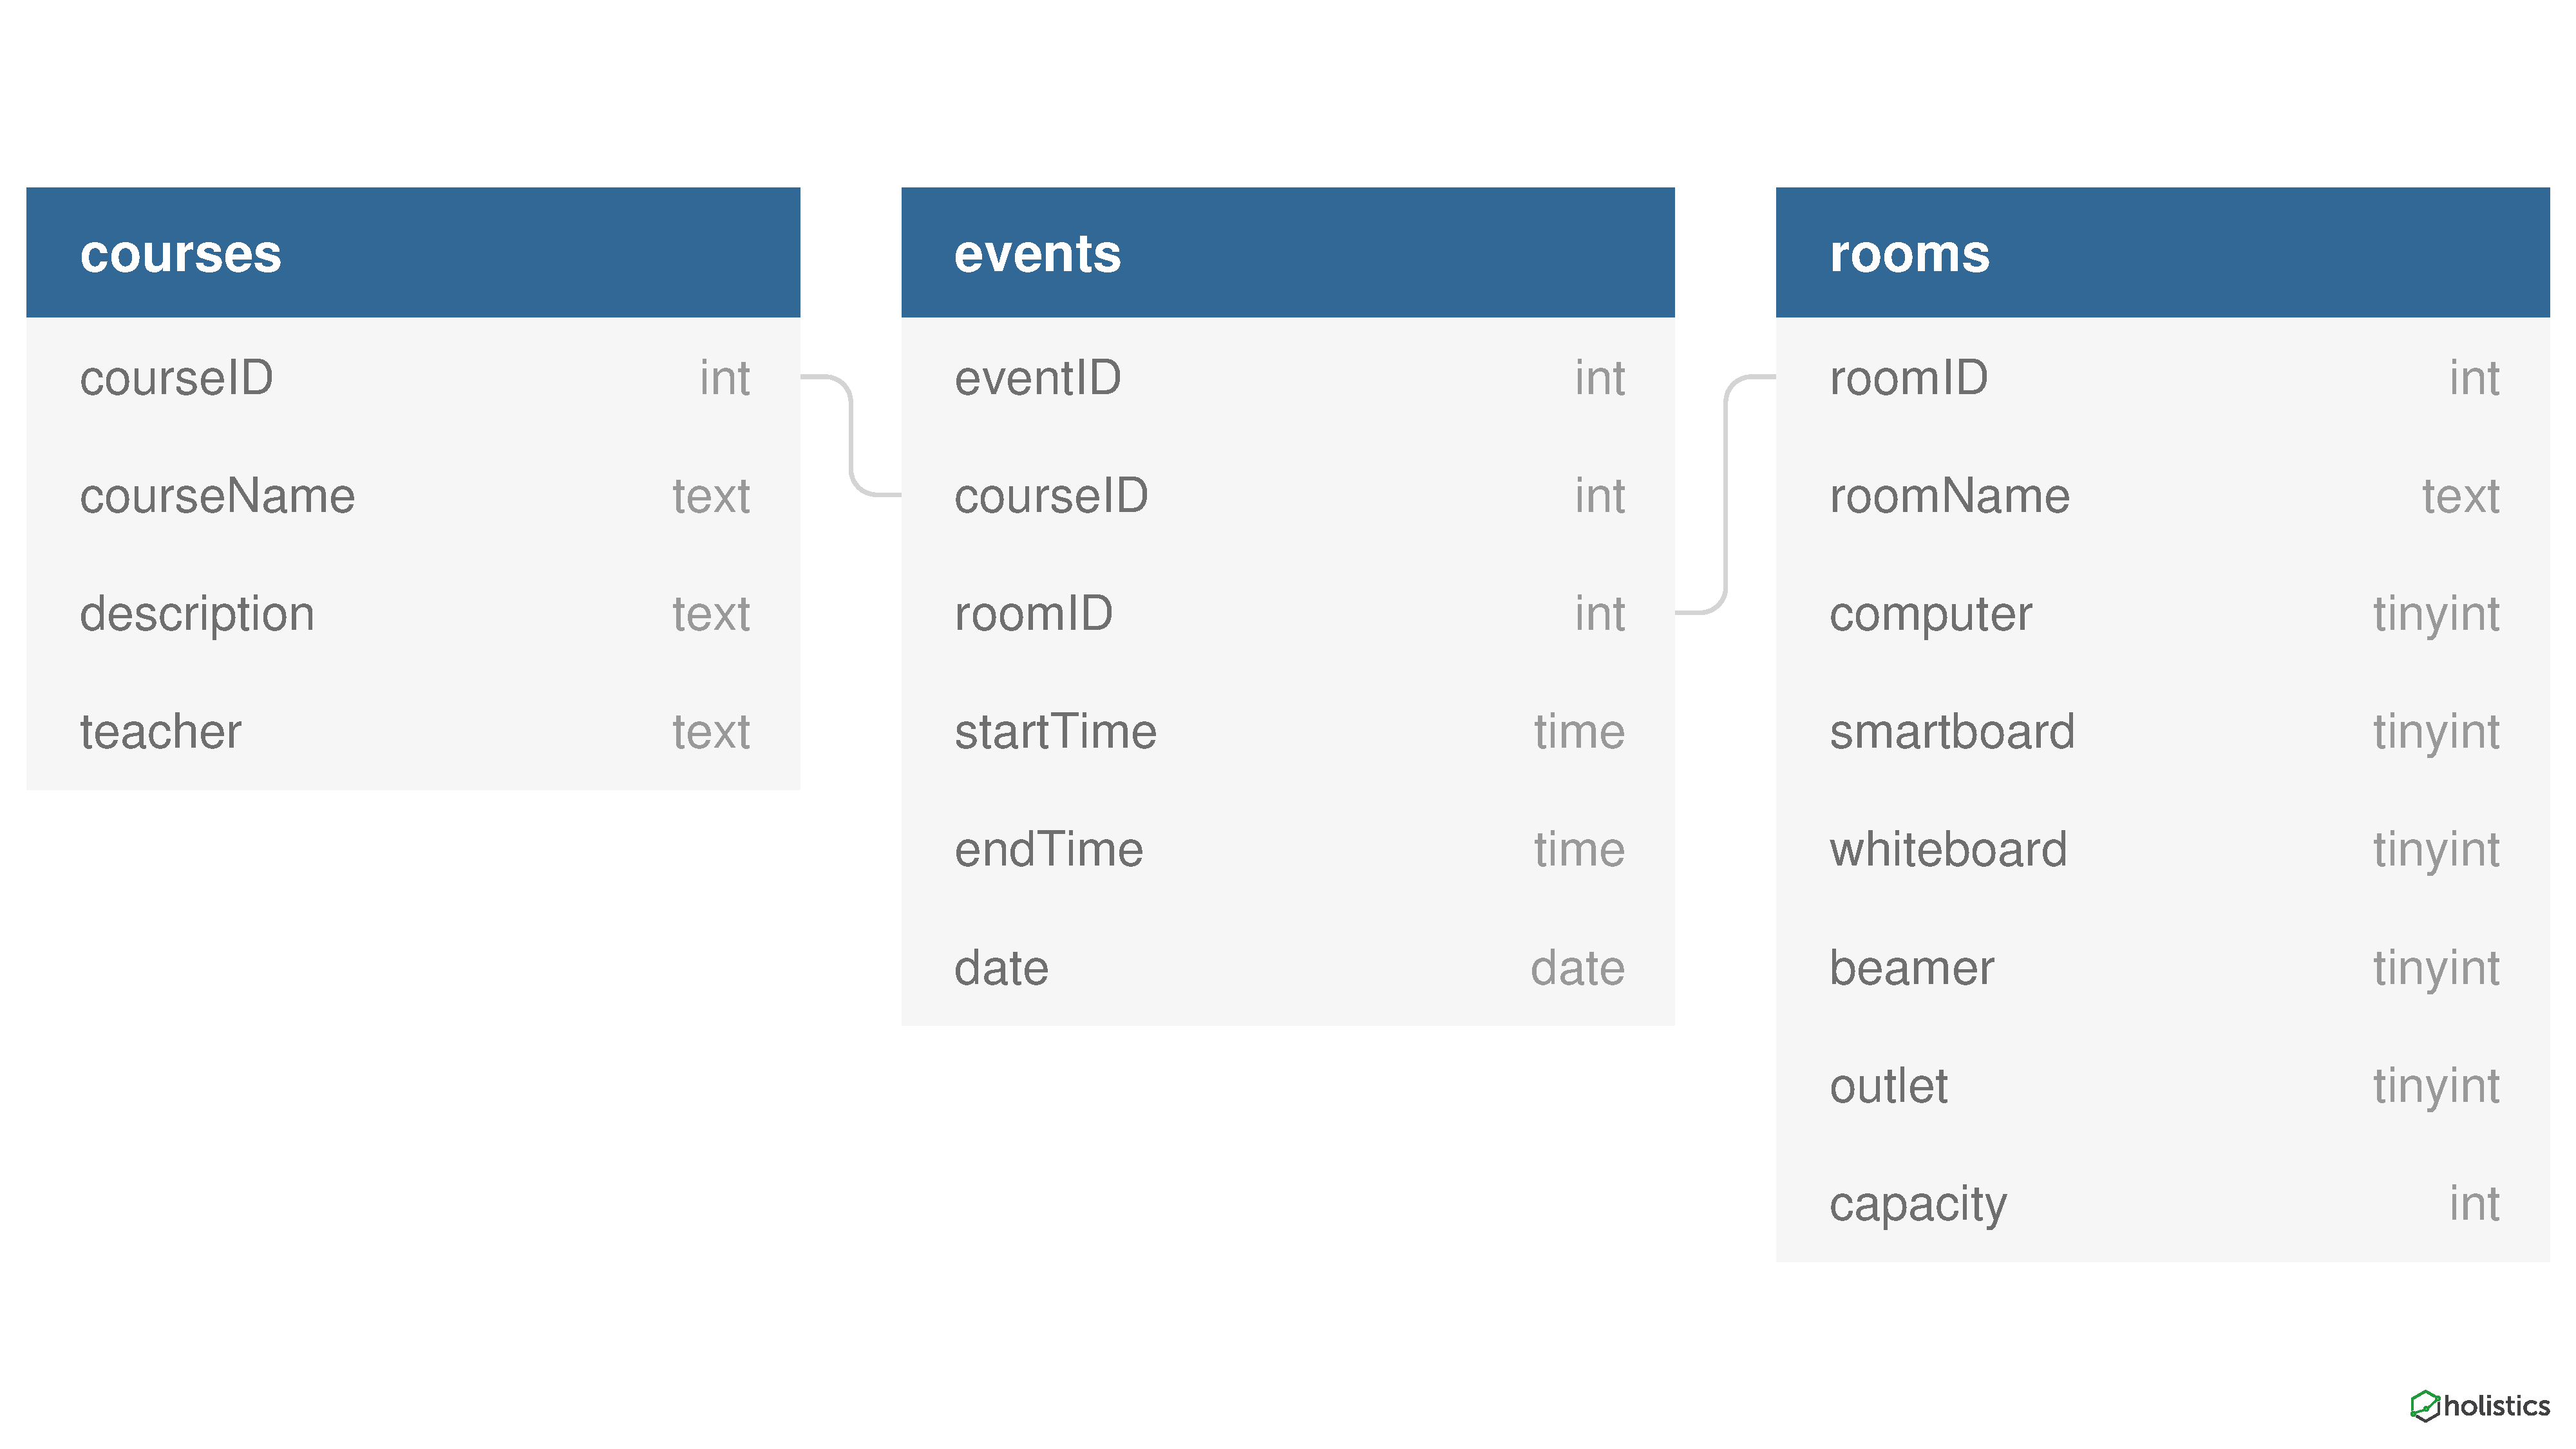
\includegraphics[width=0.9\textwidth]{dbstruct}
	\caption{Database structure}
	\label{fig:dbstruct}
\end{figure}
\subsubsection{Wifi Access Point op Raspberry Pi}
Voor het opzetten van de WAP op de Raspberry Pi hebben we een online step-by-step guide gevolgd \cite{RaspberryPiWAP}.
\subsubsection{Webserver en GET request}
\newpage

\section{Resultaten}

Wanneer we uit de databank de info van het lokaal 02.85 filteren, krijgen we volgende figuur \ref{fig:vboutput}.

\begin{figure}
	\centering
	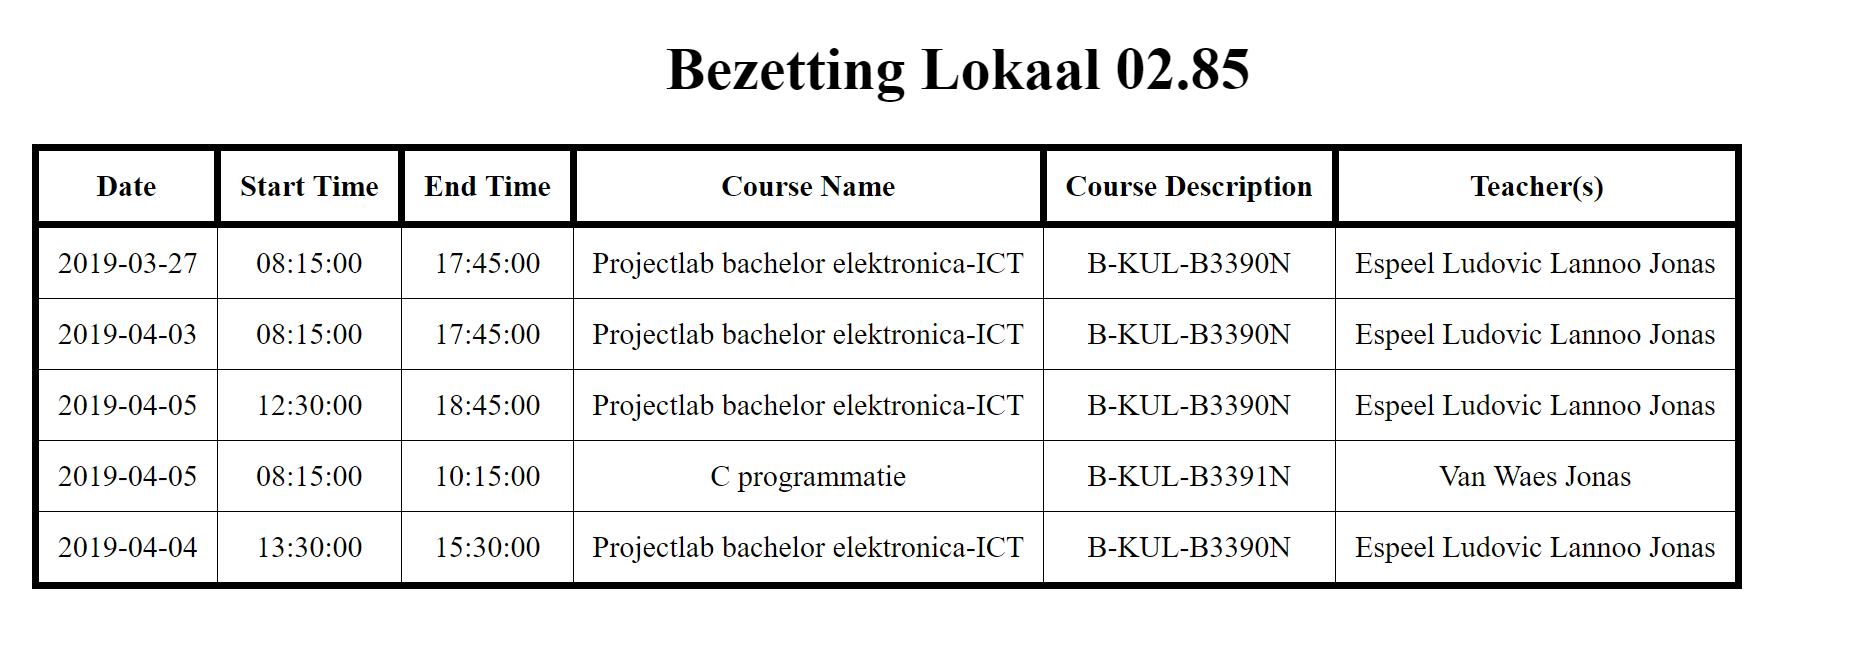
\includegraphics[width=0.75\textwidth]{vbDatabank}
	\caption{lokaalbezetting lokaal 02.85}
	\label{fig:vboutput}
\end{figure}
	
\newpage

\section{In het vervolg}

Als we dit project verder zouden uitwerken, zouden we een andere mbed en wifi module gebruiken. Nu hebben we veel tijd verloren met het zoeken naar hoe we iets moeten implementeren. We zouden kunnen werken met modules die we kennen, waardoor alles sneller zou kunnen gaan. 

\newpage

\section{Conclusie}

tekst.

\newpage

\bibliographystyle{plain}
\bibliography{library}

\end{document}
